\documentclass[11pt,letterpaper]{article}
\usepackage[utf8]{inputenc}
\usepackage[spanish]{babel}
\usepackage{amsmath}
\usepackage{amsfonts}
\usepackage{amssymb}
\usepackage{graphicx}
\usepackage{physics}
\usepackage{hyperref}
\usepackage[left=2cm,right=2cm,top=2cm,bottom=2cm]{geometry}

\usepackage[draft,inline,nomargin]{fixme} \fxsetup{theme=color}
\definecolor{jacolor}{RGB}{200,40,0} \FXRegisterAuthor{ja}{aja}{\color{jacolor}JA}

\newcommand{\mcM}{\mathcal{M}}

\renewcommand{\labelenumii}{\arabic{enumi}.\arabic{enumii}}
\renewcommand{\labelenumiii}{\arabic{enumi}.\arabic{enumii}.\arabic{enumiii}}
\renewcommand{\labelenumiv}{\arabic{enumi}.\arabic{enumii}.\arabic{enumiii}.\arabic{enumiv}}

%%%%% Author
\author{José Alfredo de León}

%%%% Title 
\title{Tarea 2\\
\large{Métodos de Simulación Computacional para Sistemas Cuánticos - 2022-2}}


\begin{document}
\date{24 de febrero de 2022}
\maketitle

\section{Objetivos}

\subsection{Objetivo general}
Implementar en Mathematica 
los algoritmos de interpolación polinomial y splines (lineal y cúbico) y
comparar cuál de estos métodos numéricos es el más útil.

\subsection{Objetivos específicos}
\begin{enumerate}
\item Utilizar la rutina de eliminación de Gauss-Jordan implementada en 
la tarea 1.
\item Investigar numéricamente cómo se comportan la interpolación polinomial
e interpolación de splines para conjuntos de datos con espacimiento regular
y aleatorio.
\end{enumerate}

\section{El problema}
Para esta tarea implementamos e investigamos numéricamente algunos 
de los métodos que existen para interpolación. La interpolación es el proceso
de estimar valores desconocidos dentro de intervalos cuyos extremos son
conocidos. En particular, en esta sección describiremos brevemente dos métodos:
intepolación polinomial y el método por secciones de \textit{splines}.

Por un lado, el método de interpolación polinomial es un método en el que
se tiene como objetivo aproximar una función $f(x)$ mediante un polinomio 
en el rango de los valores de $x$ \cite{cohen2011numerical}. Si se tienen $n$ puntos
$x_i,y_i)$, entonces se puede aproximar la función analítica
$f(x)$ que conecta los puntos con un polinomio de la forma
\begin{align}\label{eq:interpolation_poly}
f(x)=a_0+a_1x+a_2x^2+\ldots+a_{n-1}x^{n-1}.
\end{align}

Dado el conjunto $\{\big(x_i,y_i\}$ ($0\leq i\leq n-1$) se construye el sistema 
lineal de ecuaciones con los $n$ coeficientes $a_i$ indeterminados
\begin{align}\label{eq:interpolation_poly_matrix}
\mqty(
1&x_1&x_1^2&\ldots&x_{1}^{n-1}\\
\vdots&\vdots&\vdots&\ddots&\vdots\\
1&x_n&x_n^2&\ldots&x_{n}^{n-1}\\)
\mqty(
a_0\\
\vdots\\
a_{n-1}
)
=
\mqty(
y_0\\
\vdots\\
y_{n-1}
),
\end{align}
De aquí en adelante el problema de construir el polinomio de interpolación
se ha reducido a resolver el sistema \eqref{eq:interpolation_poly_matrix} para
encontrar los coeficientes $a_i$ de \eqref{eq:interpolation_poly}. 

%\janote{Hablar sobre interpolación de splienes. Citar el libro de numerical 
%nos é que de Bryan}
Por otro lado, la interpolación por secciones de \textit{splines} consiste en,
dado un conjunto $\{\big(x_i,y_i)\}$ ($1\leq i\leq n$), conectar
cada intervalo $x_i\leq x\leq x_{i+1}$ ($1\leq i \leq n-1$) con un polinomio
para aproximar la función analítica que conecta a todos los puntos en el intervalo
$x_1\leq x\leq x_n$. Es decir, a diferencia de la interpolación polinomial,
en la interpolación por secciones de \textit{splines} aproxima a la función
analítica con una función definida a trozos, con un polinomio en cada interavalo.

Uno de los métodos más sencillos de \textit{splines} es el de aproximar
la función analítica que conecta todos los puntos del conjunto con 
un polinomio lineal entre puntos consecutivos del conjunto como~\cite{cohen2011numerical}
\begin{align}
f(x)=a_ix+b_i,\quad x_i\leq x\leq x_{i+1}
\end{align}
Para calcular los coeficientes $a_i$ y $b_i$ se utilizan las siguientes expresiones
\begin{align}
a_i&=\frac{y_{i+1}-y_i}{x_{i+1}-x_i},& b_i=&y_i-a_ix_i.
\end{align}
No obstante, el método de interpolación por secciones de \textit{splines} lineales
no es realmente útil en la práctica dado que la función definida a trozos
con este aproximación no es una función suave, es decir, su primera derivada
no es continua en cada uno de los puntos del conjunto de datos.

La interpolación por secciones de \textit{splines} más comúnmente utilizada
es de los \textit{splines} cúbicos. Un ventaja de los \textit{splines} cúbicos frente
a los lineales es que aproximan a la función $f(x)$ con una función suave, es decir,
una función definida a trozos cuyas primera y segunda derivada son continuas 
para cada punto de la función.

La función construída con \textit{splines} cúbicos es de la forma
\begin{align}
f(x)=a_i+b_i(x-x_i)+c_i(x-x_i)^2+d_i(x-x_i)^3,\quad x_i\leq x\leq x_{i+1}.
\end{align}

Si bien en este manuscrito no discutiremos en detalle la derivación del
cálculo de los valores de las constantes $b_i$, $c_i$ y $d_i$, sólo presentaremos
un resumen de la derivación de Burden y Faires \cite{burden2015numerical}:
%\janote{Exponer las condiciones 1de los splines}
\begin{itemize}
\item $a_i=y_i$ ya que $f(x_i)=a_i$.
\item Para encontrar los valores de las constantes $c_i$ se debe de resolver 
el sistema de ecuaciones lineal
\begin{align}
\mathcal{A}\vec c=\vec \alpha,
\end{align}
donde 
\begin{align}\label{eq:A_y_b_cubic_spine}
\mathcal{A}&=
\mqty(
1&0&0&\ldots&\ldots&0\\
h_1&2(h_1+h_2)&h_2&\ddots&&\vdots\\
0&h_2&2(h_2+h_3)&h_3&\ddots&\vdots\\
\vdots&\ddots&\ddots&\ddots&\ddots&0\\
\vdots&&\ddots&h_{n-2}&2(h_{n-2}+h_{n-1})&h_{n-1}\\
0&\ldots&\ldots&0&0&1
)\\
\end{align}
y
\begin{align}
\vec \alpha&=
\mqty(
0\\
\frac{3}{h_2}\qty(a_3-a_2)-\frac{3}{h_1}\qty(a_2-a_1)\\
\vdots\\
\frac{3}{h_n}\qty(a_{n+1}-a_{n})-\frac{3}{h_{n-1}}\qty(a_{n}-a_{n-1})\\
0
).
\end{align}
\item Para calcular $b_j$
\begin{align}
b_i=\frac{1}{h_i}\qty(a_{i+1}-a_i)-\frac{h_i}{3}\qty(2c_i+c_{i+1})
\end{align}
\item Finalmente, para calcular $d_i$ se usa
\begin{align}
d_i=\frac{c_{i+1}-c_i}{3h_i}
\end{align}
\end{itemize}

\subsection{El problema de la tarea}
Para esta tarea comparamos los tres métodos 
de interpolación que presentamos en la sección anterior para conjuntos de 
16, 32 y 64 puntos con espaciamiento regular y aleatorio en en los intervalos
$[0,2\pi]$, para la función $f(x)=2\cos (x)+\sin (x)+\sqrt{x}$, y
$[0,1]$ para la función $f(x)=2\cos (2\pi x)+\sin (2\pi x)+\sqrt{2\pi x}$.

\section{Implementación}
%\janote{echar una última revisada si se puede}
En esta sección enunciamos los algoritmos que fueron implementados en 
Mathematica para los tres siguientes métodos:
\begin{enumerate}
\item Polinomio de interpolación
\item Spline lineal
\item Spline cúbico 
\end{enumerate}

\subsection{Polinomio de interpolación}
\textbf{Entrada}: (1) Lista $x$ con los valores $x_i$ del conjunto de datos $\{(x_i,y_i)\}$;
y (2) lista $y$ con los valores $y_i$ del conjunto de datos $\{(x_i,y_i)\}$.

\textbf{Salida}: Lista $\vec a$ con las soluciones de los coeficientes $a_i$ del polinomio 
de interpolación.

\textbf{Necesita}: Rutinas \textit{GaussJordan} y \textit{GaussJordanSolution}\footnote{
\textit{GaussJordanSolution es una nueva rutina para ordenar las soluciones
de la rutina \textit{GaussJordan}} % \janote{Explicar algoritmo?}
}.
\begin{enumerate}
\item Construir la matriz aumentada $(\mathcal{X}|b)$ del sistema 
de ecuaciones lineales con los coeficientes del polinomio de interpolación
como incógnitas.
\item Hacer eliminación de Gauss-Jordan a la matriz aumentada $(\mathcal{X}|b)$.
\item Construir el vector $\vec a$ de soluciones de los coeficientes $a_i$
del polinomio de interpolación.
\end{enumerate}

\subsection{Spline lineal}
\textbf{Entrada}: (1) lista con los valores $x_i$ ($1\leq i\leq n$), (2)
lista con los valores $y_i$ ($1\leq i\leq n$); ; (3) variable
simbólica ($x$ por ejemplo) en función de la cual se definirá la función 
con los splines; y (4) número ``1'' que indica el grado de los
splines.

\textbf{Salida}: función a trozos con cada spline lineal conectando a dos puntos
consecutivos del conjunto de datos.

\begin{enumerate}
\item Calcular $\alpha_k=(y_{k+1}-y_k)/(x_{k+1}-x_k)$.
\item Calcular $\beta_k=y_k-\alpha_k x_k$.
\item Definir la función a trozos $f(x)=\alpha_k x+\beta_k,\quad x_k\leq x\leq x_{k+1},
\quad k=0,\ldots,n-1$.
\end{enumerate}

\subsection{Spline cúbico}
\textbf{Entrada}: (1) lista con los valores $x_i$ ($1\leq i\leq n$), (2)
lista con los valores $y_i$ ($1\leq i\leq n$); ; (3) variable
simbólica ($x$ por ejemplo) en función de la cual se definirá la función 
con los splines; y (4) número ``3'' que indica el grado de los
splines.

\textbf{Salida}: función a trozos con cada spline lineal conectando a dos puntos
consecutivos del conjunto de datos

\textbf{Necesita}: \textit{GaussJordan} y \textit{GaussJordanSolution}.

\begin{enumerate}
\item Calcular los coeficientes $a_i=y_i$ ($1\leq i\leq n-1$).
\item Calcular $h_i=x_{i+1}-x_i$ ($1\leq i\leq n-1$).
\item Construir la matriz aumentada $\big( A\big|\vec b\big)$, $A$ y
$\vec b$ definidas en \eqref{eq:A_y_b_cubic_spine}.
\item Resolver la matriz aumentada  $\big( A\big|\vec b\big)$ 
mediante eliminación de Gauss-Jordan.
\item Calcular $b_j=1/h(y_{i+1}-y_i)-h/3(2c_i+c_{i+1})$ ($1\leq i\leq n$).
\item Calcular los coeficientes $d_i=(c_{i+1}-c_i)/3h$ ($1\leq i\leq n$).
\item Definir la función a trozos 
$f(x)=a_i+b_ix+c_ix^2+d_ix^3,
\quad x_i\leq x\leq x_{i+1},
\quad i=1,\ldots,n-1$
\end{enumerate}


\section{Parte 1: Polinomio de interpolación}
Los resultados se muestran de la fig. \ref{fig1} a la fig.\ref{fig12}.

\begin{figure} 
\centering
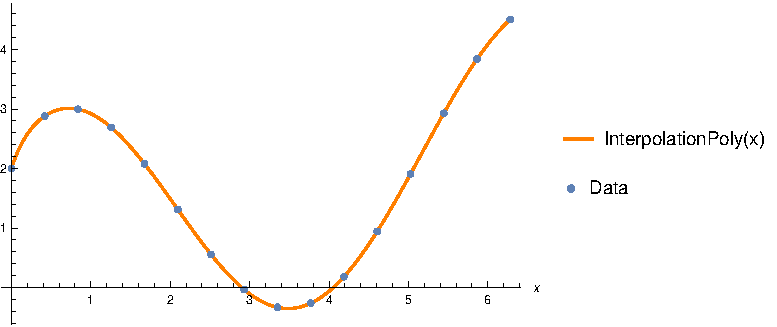
\includegraphics[width=10cm]{img/1.pdf}
\caption{Interpolación polinomial. $f(x)=2\cos (x)+\sin (x)+\sqrt{x}$, 16 puntos especiados regularmente.}
\label{fig1}
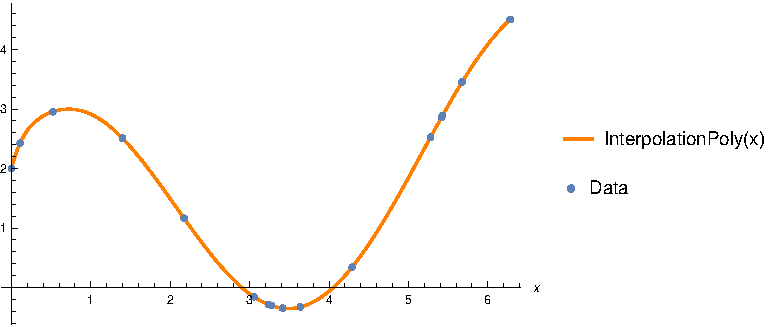
\includegraphics[width=10cm]{img/2.pdf}
\caption{Interpolación polinomial. $f(x)=2\cos (x)+\sin (x)+\sqrt{x}$, 16 puntos espaciados aleatoriamente.}
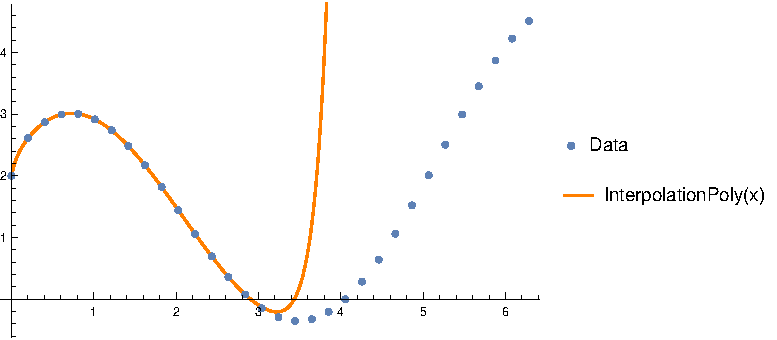
\includegraphics[width=10cm]{img/3.pdf}
\caption{Interpolación polinomial. $f(x)=2\cos (x)+\sin (x)+\sqrt{x}$, 32 puntos especiados regularmente.}
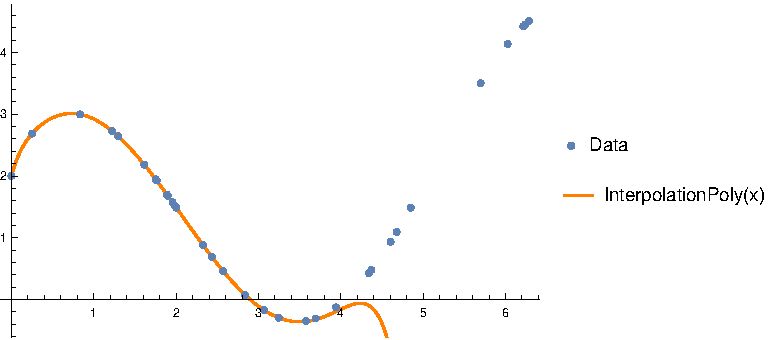
\includegraphics[width=10cm]{img/4.pdf}
\caption{Interpolación polinomial. $f(x)=2\cos (x)+\sin (x)+\sqrt{x}$, 32 puntos espaciados aleatoriamente.}
\end{figure}


\begin{figure}
\centering
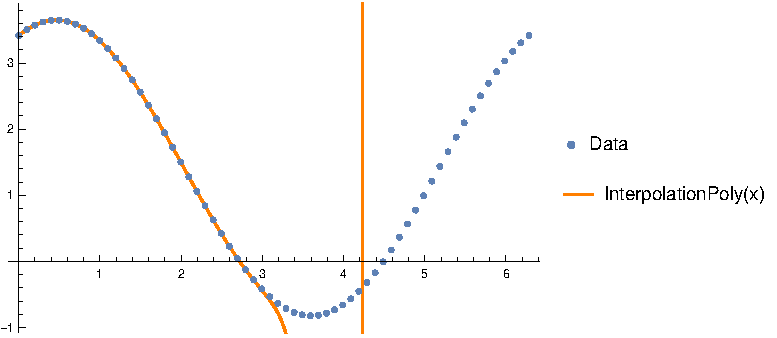
\includegraphics[width=10cm]{img/5.pdf}
\caption{Interpolación polinomial. $f(x)=2\cos (x)+\sin (x)+\sqrt{x}$, 64 puntos especiados regularmente.}
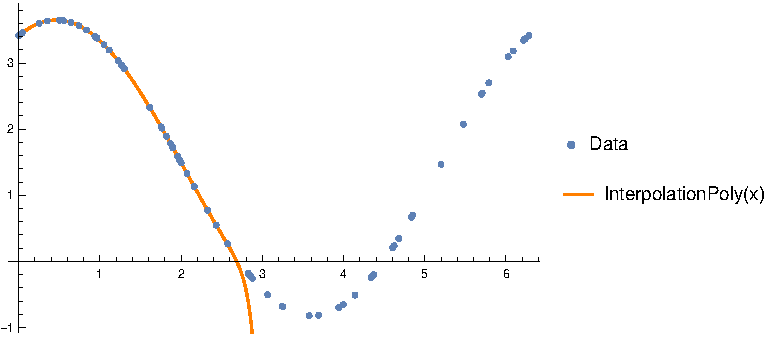
\includegraphics[width=10cm]{img/6.pdf}
\caption{Interpolación polinomial. $f(x)=2\cos (x)+\sin (x)+\sqrt{x}$, 64 puntos espaciados aleatoriamente.}
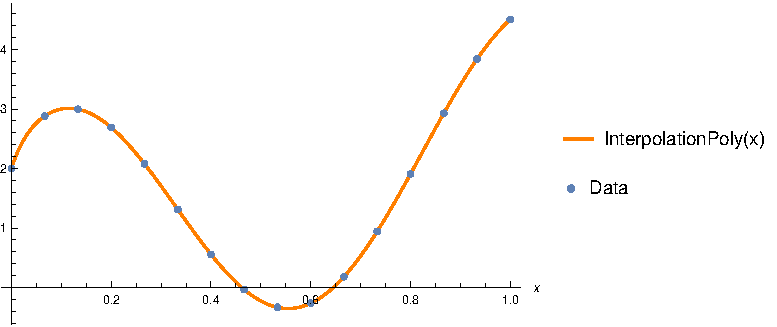
\includegraphics[width=10cm]{img/7.pdf}
\caption{Interpolación polinomial. $f(x)=2\cos (2\pi x)+\sin (2\pi x)+\sqrt{2\pi x}$, 16 puntos especiados regularmente.}
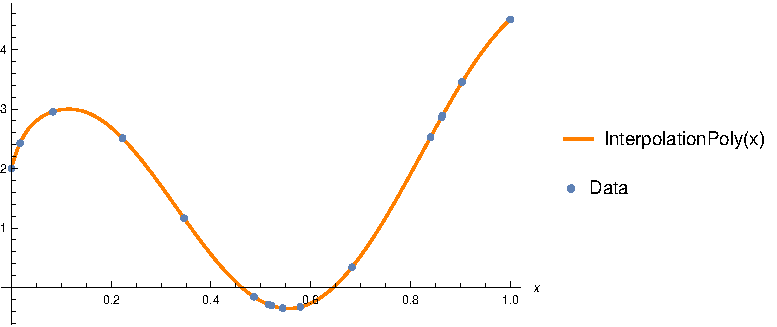
\includegraphics[width=10cm]{img/8.pdf}
\caption{Interpolación polinomial. $f(x)=2\cos (2\pi x)+\sin (2\pi x)+\sqrt{2\pi x}$, 16 puntos espaciados aleatoriamente.}
\end{figure}

\begin{figure}
\centering
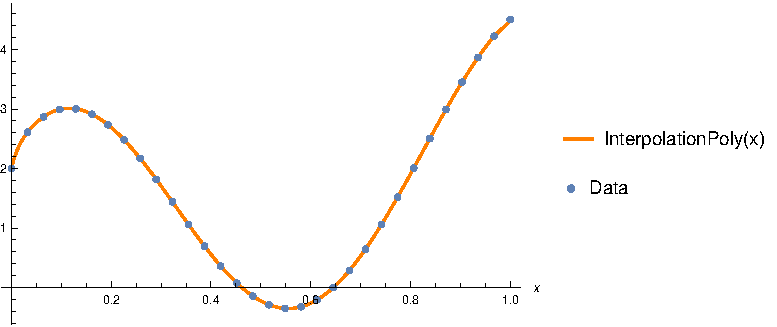
\includegraphics[width=10cm]{img/9.pdf}
\caption{Interpolación polinomial. $f(x)=2\cos (2\pi x)+\sin (2\pi x)+\sqrt{2\pi x}$, 32 puntos especiados regularmente.}
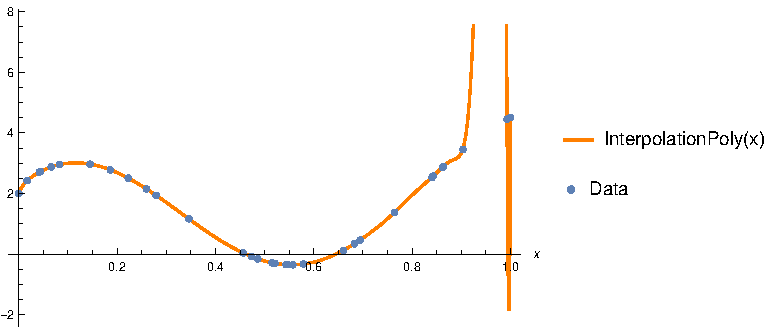
\includegraphics[width=10cm]{img/10.pdf}
\caption{Interpolación polinomial. $f(x)=2\cos (2\pi x)+\sin (2\pi x)+\sqrt{2\pi x}$, 32 puntos espaciados aleatoriamente.}
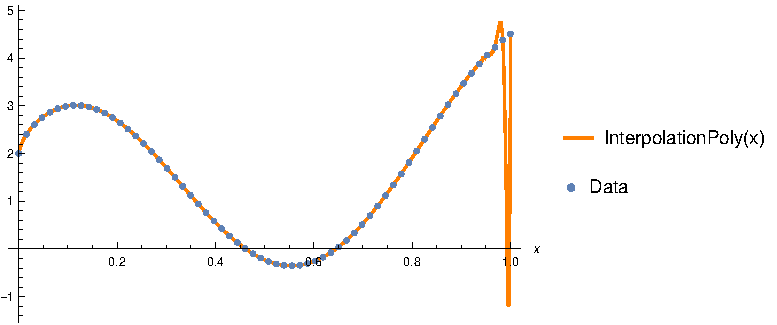
\includegraphics[width=10cm]{img/11.pdf}
\caption{Interpolación polinomial. $f(x)=2\cos (2\pi x)+\sin (2\pi x)+\sqrt{2\pi x}$, 64 puntos especiados regularmente.}
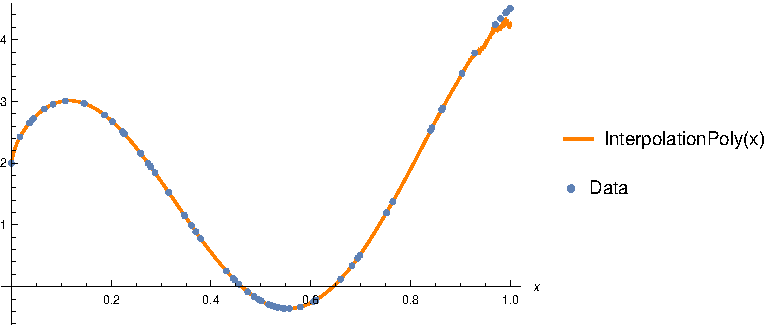
\includegraphics[width=10cm]{img/12.pdf}
\caption{Interpolación polinomial. $f(x)=2\cos (2\pi x)+\sin (2\pi x)+\sqrt{2\pi x}$, 64 puntos espaciados aleatoriamente.}
\label{fig12}
\end{figure}

\section{Parte 2: Interpolación por secciones, splines}
Los resultados se muestran de la fig. \ref{fig13} a la fig.\ref{fig36}.
\begin{figure}
\centering
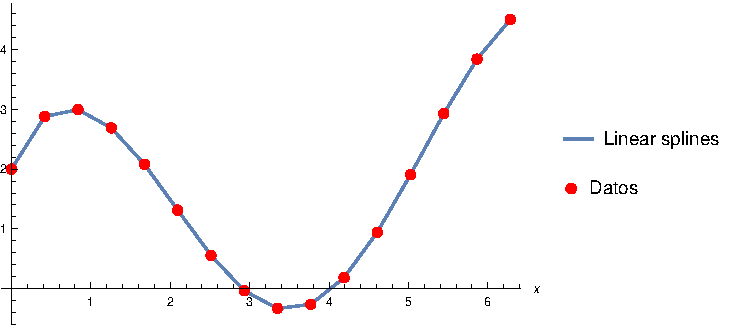
\includegraphics[width=10cm]{img/13.pdf}
\caption{Splines lineales. $f(x)=2\cos (x)+\sin (x)+\sqrt{x}$, 16 puntos especiados regularmente.}
\label{fig13}
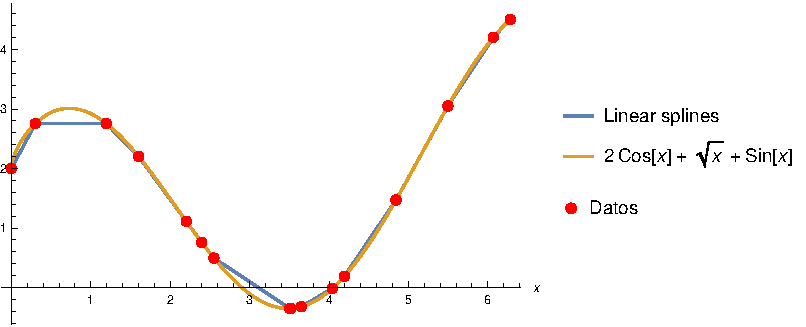
\includegraphics[width=10cm]{img/14.pdf}
\caption{Splines lineales. $f(x)=2\cos (x)+\sin (x)+\sqrt{x}$, 16 puntos espaciados aleatoriamente.}
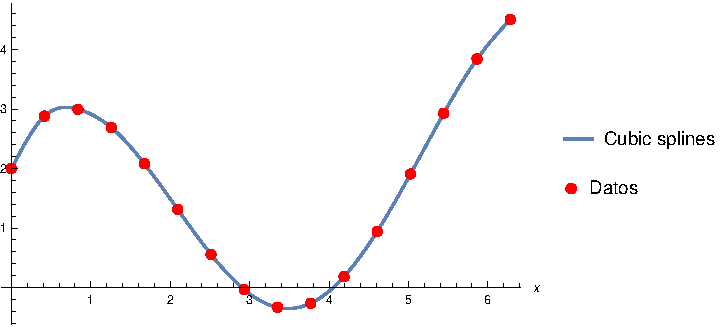
\includegraphics[width=10cm]{img/15.pdf}
\caption{Splines cúbicos. $f(x)=2\cos (x)+\sin (x)+\sqrt{x}$, 16 puntos especiados regularmente.}
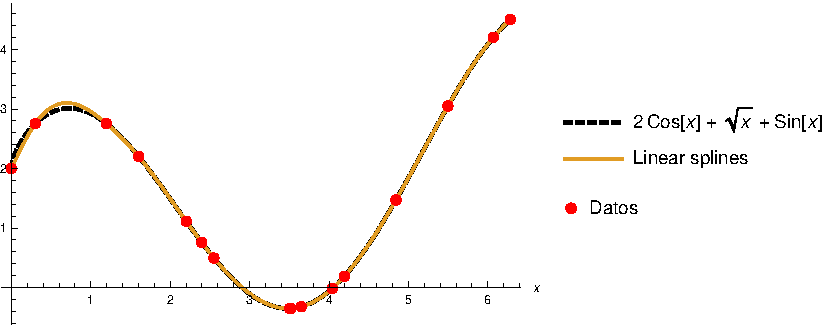
\includegraphics[width=10cm]{img/16.pdf}
\caption{Splines cúbicos. $f(x)=2\cos (x)+\sin (x)+\sqrt{x}$, 16 puntos espaciados aleatoriamente.}
\end{figure}

\begin{figure}
\centering
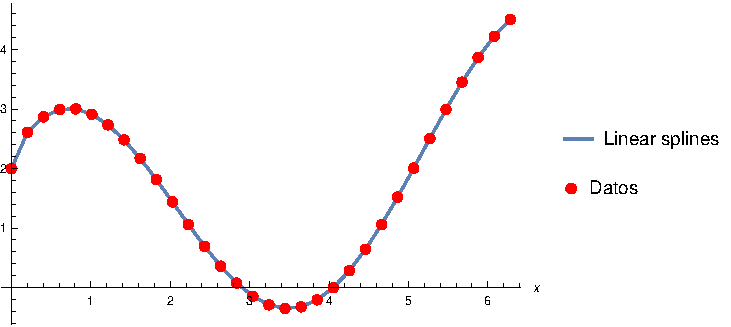
\includegraphics[width=10cm]{img/17.pdf}
\caption{Splines lineales. $f(x)=2\cos (x)+\sin (x)+\sqrt{x}$, 32 puntos especiados regularmente.}
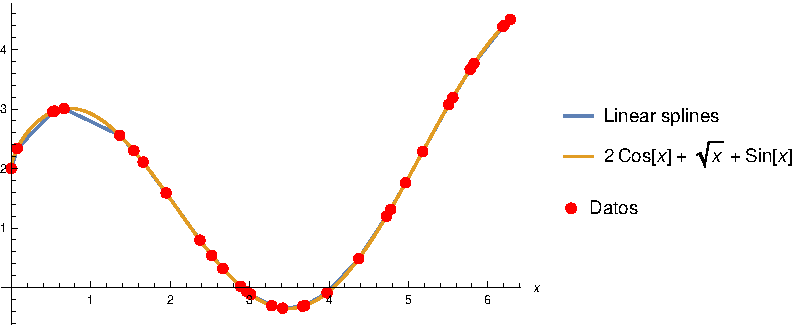
\includegraphics[width=10cm]{img/18.pdf}
\caption{Splines lineales. $f(x)=2\cos (x)+\sin (x)+\sqrt{x}$, 32 puntos espaciados aleatoriamente.}
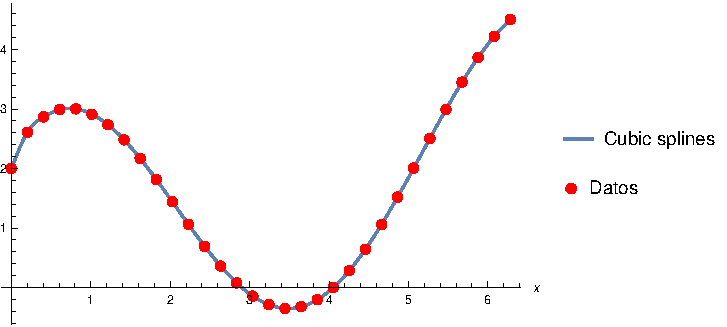
\includegraphics[width=10cm]{img/19.pdf}
\caption{Splines cúbicos. $f(x)=2\cos (x)+\sin (x)+\sqrt{x}$, 32 puntos especiados regularmente.}
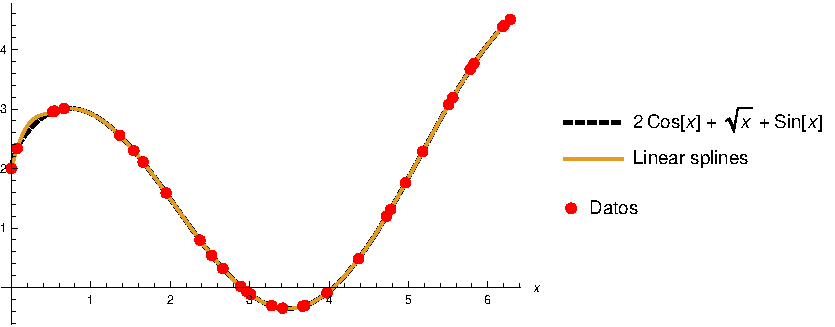
\includegraphics[width=10cm]{img/20.pdf}
\caption{Splines cúbicos. $f(x)=2\cos (x)+\sin (x)+\sqrt{x}$, 32 puntos espaciados aleatoriamente.}
\end{figure}

\begin{figure}
\centering
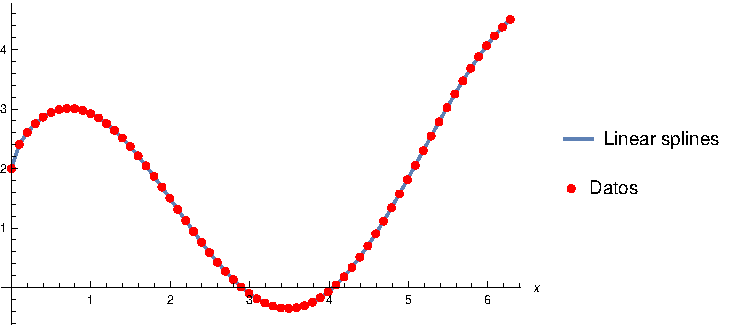
\includegraphics[width=10cm]{img/21.pdf}
\caption{Splines lineales. $f(x)=2\cos (x)+\sin (x)+\sqrt{x}$, 64 puntos especiados regularmente.}
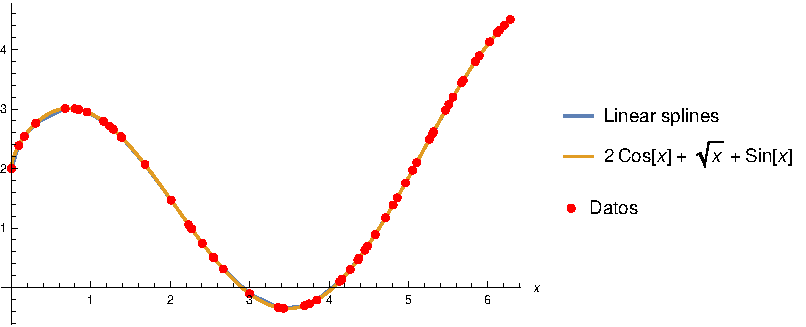
\includegraphics[width=10cm]{img/22.pdf}
\caption{Splines lineales. $f(x)=2\cos (x)+\sin (x)+\sqrt{x}$, 64 puntos espaciados aleatoriamente.}
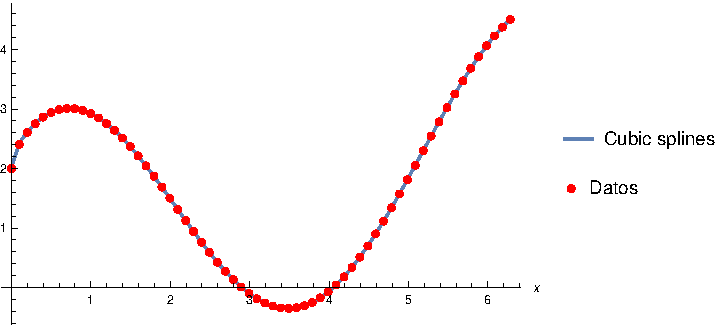
\includegraphics[width=10cm]{img/23.pdf}
\caption{Splines cúbicos. $f(x)=2\cos (x)+\sin (x)+\sqrt{x}$, 64 puntos especiados regularmente.}
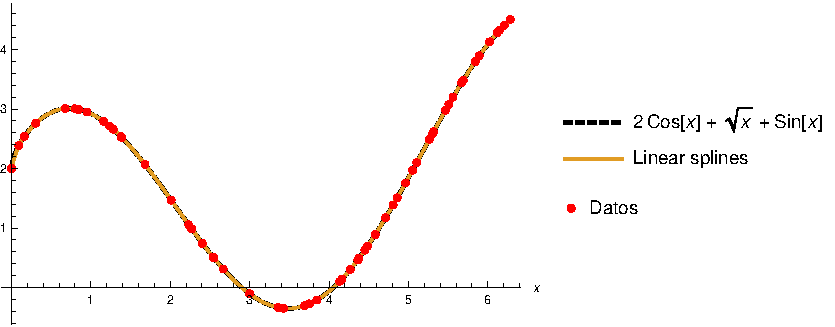
\includegraphics[width=10cm]{img/24.pdf}
\caption{Splines cúbicos. $f(x)=2\cos (x)+\sin (x)+\sqrt{x}$, 64 puntos espaciados aleatoriamente.}
\end{figure}

\begin{figure}
\centering
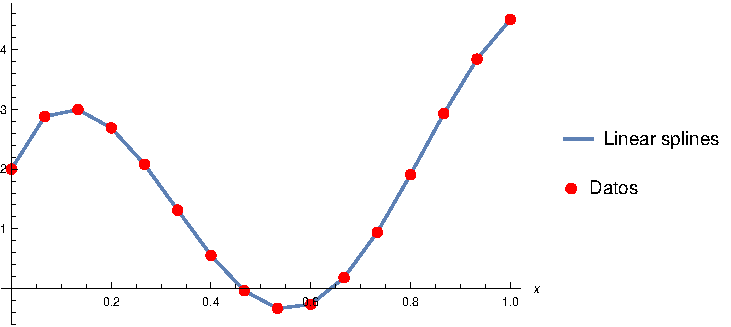
\includegraphics[width=10cm]{img/25.pdf}
\caption{Splines lineales. $f(x)=2\cos (2\pi x)+\sin (2\pi x)+\sqrt{2\pi x}$, 16 puntos especiados regularmente.}
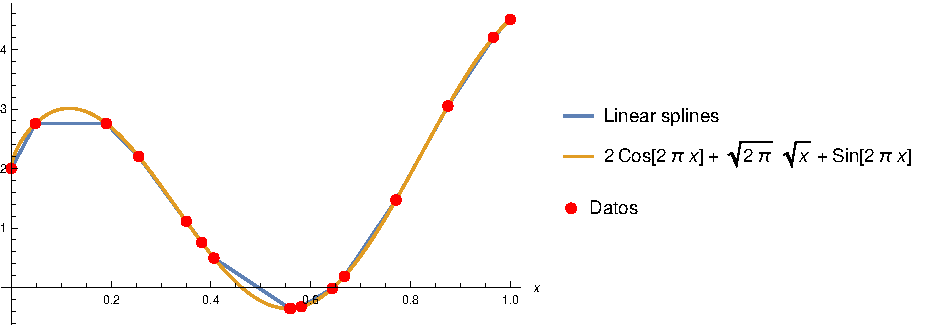
\includegraphics[width=10cm]{img/26.pdf}
\caption{Splines lineales. $f(x)=2\cos (2\pi x)+\sin (2\pi x)+\sqrt{2\pi x}$, 16 puntos espaciados aleatoriamente.}
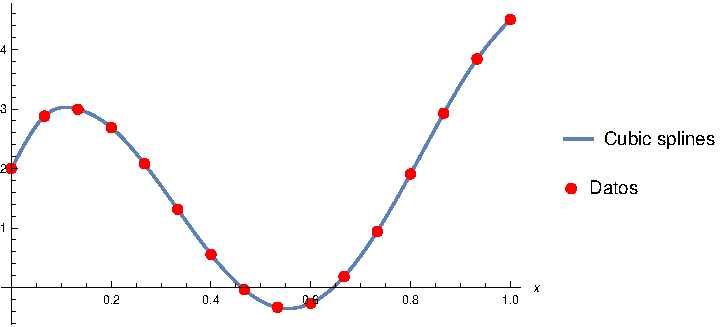
\includegraphics[width=10cm]{img/27.pdf}
\caption{Splines cúbicos. $f(x)=2\cos (2\pi x)+\sin (2\pi x)+\sqrt{2\pi x}$, 16 puntos especiados regularmente.}
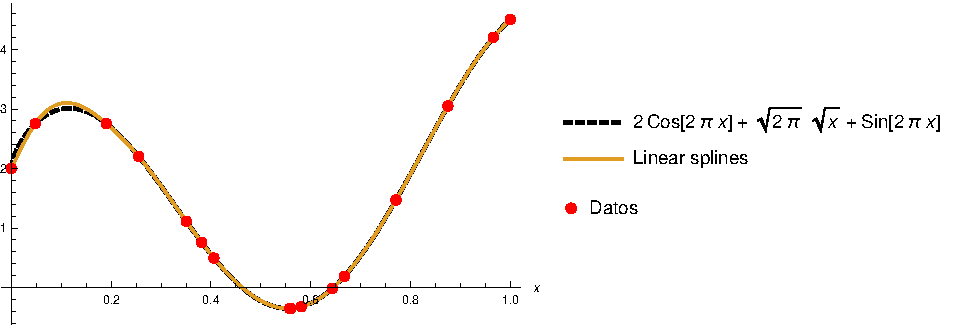
\includegraphics[width=10cm]{img/28.pdf}
\caption{Splines cúbicos. $f(x)=2\cos (2\pi x)+\sin (2\pi x)+\sqrt{2\pi x}$, 16 puntos espaciados aleatoriamente.}
\end{figure}


\begin{figure}
\centering
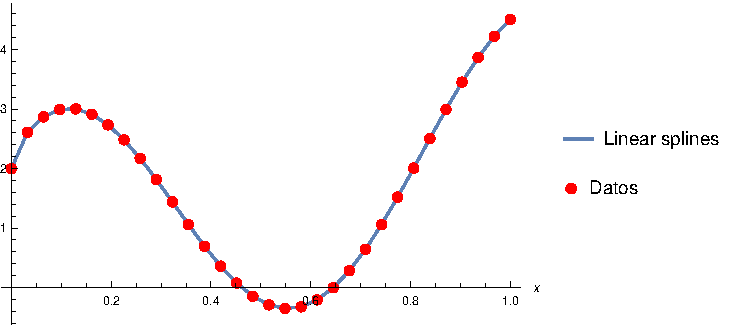
\includegraphics[width=10cm]{img/29.pdf}
\caption{Splines lineales. $f(x)=2\cos (2\pi x)+\sin (2\pi x)+\sqrt{2\pi x}$, 32 puntos especiados regularmente.}
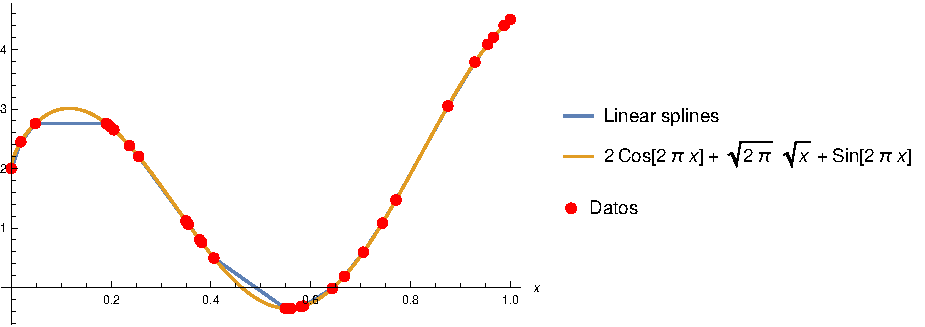
\includegraphics[width=10cm]{img/30.pdf}
\caption{Splines lineales. $f(x)=2\cos (2\pi x)+\sin (2\pi x)+\sqrt{2\pi x}$, 32 puntos espaciados aleatoriamente.}
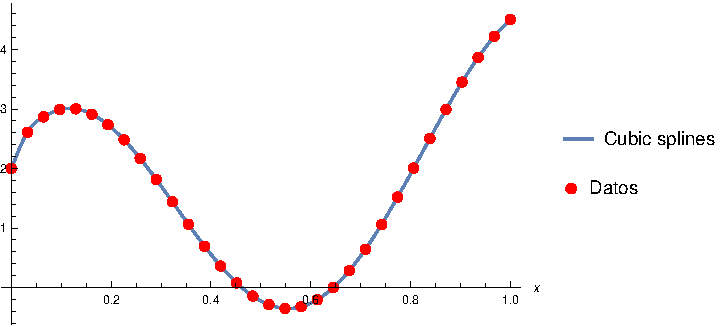
\includegraphics[width=10cm]{img/31.pdf}
\caption{Splines cúbicos. $f(x)=2\cos (2\pi x)+\sin (2\pi x)+\sqrt{2\pi x}$, 32 puntos especiados regularmente.}
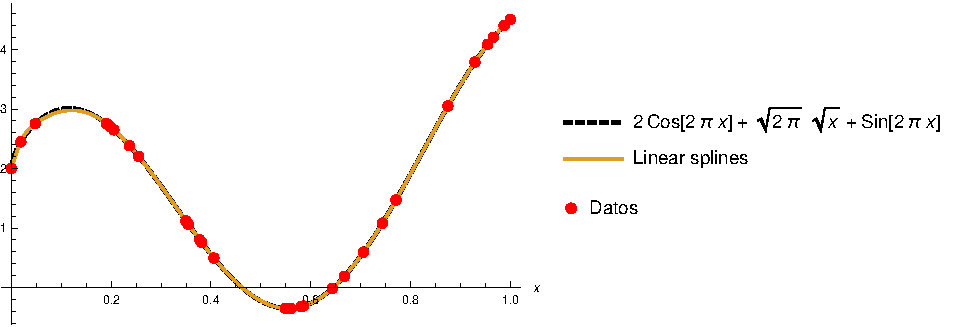
\includegraphics[width=10cm]{img/32.pdf}
\caption{Splines cúbicos. $f(x)=2\cos (2\pi x)+\sin (2\pi x)+\sqrt{2\pi x}$, 32 puntos espaciados aleatoriamente.}
\end{figure}

\begin{figure}
\centering
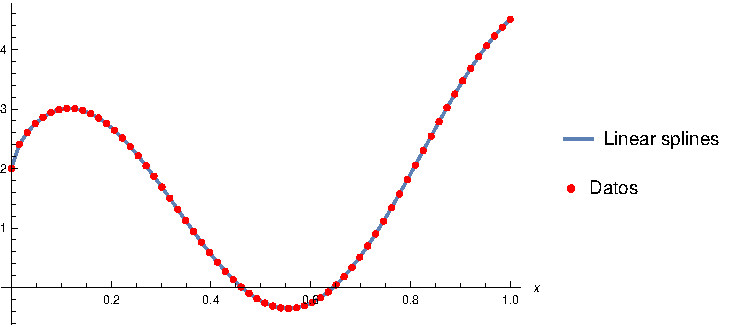
\includegraphics[width=10cm]{img/33.pdf}
\caption{Splines lineales. $f(x)=2\cos (2\pi x)+\sin (2\pi x)+\sqrt{2\pi x}$, 64 puntos especiados regularmente.}
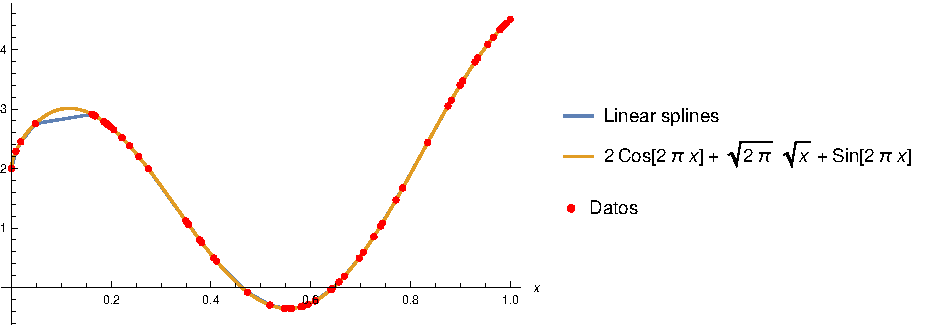
\includegraphics[width=10cm]{img/34.pdf}
\caption{Splines lineales. $f(x)=2\cos (2\pi x)+\sin (2\pi x)+\sqrt{2\pi x}$, 64 puntos espaciados aleatoriamente.}
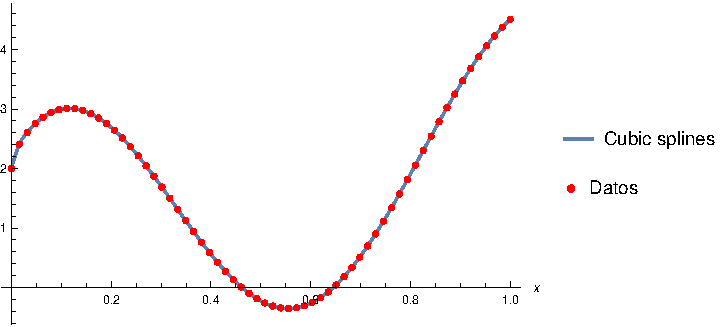
\includegraphics[width=10cm]{img/35.pdf}
\caption{Splines cúbicos. $f(x)=2\cos (2\pi x)+\sin (2\pi x)+\sqrt{2\pi x}$, 64 puntos especiados regularmente.}
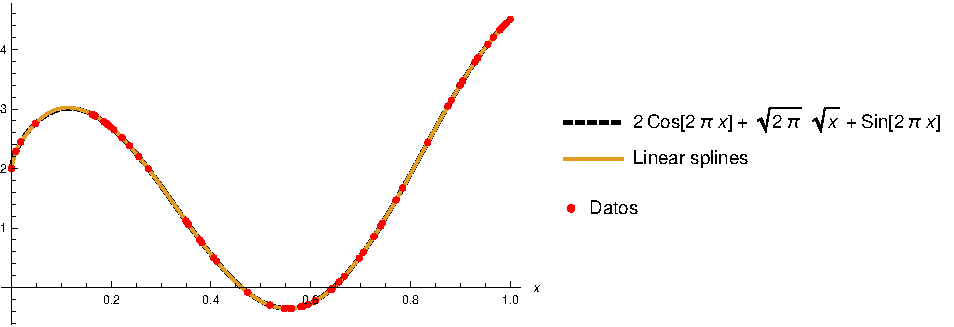
\includegraphics[width=10cm]{img/36.pdf}
\caption{Splines cúbicos. $f(x)=2\cos (2\pi x)+\sin (2\pi x)+\sqrt{2\pi x}$, 64 puntos espaciados aleatoriamente.}
\label{fig36}
\end{figure}


\section{Discusión}
Los resultados muestran que la interpolación por secciones de \textit{splines} cúbicos
son un mejor método para aproximar la función que une a los puntos de un set de 
datos. Notamos que el método de interpolación polinomial 
funciona bien para 16 puntos con espaciado regular, pero para 32 y 64
puntos con espaciado regular o aleatorio notamos, en general, que el 
método se vuelve inestable y no aproxima de manera satisfactoria la función
analítica. Por otro lado, el método de interpolación por secciones de
\textit{splines} muestra que, incluso para \textit{splines} lineales, se consigue
una mejor aproximación de la función analítica que con el método de 
interpolación polinomial para cantidad de puntos con espaciado regular
o aleatorio. Un problema que se notó en los resultados, además de 
la no continuidad de los \textit{splines} lineales que \textit{apriori}
se conoce, es que para puntos espaciados aleatoriamente los \textit{splines}
lineales ya no aproximan satisfactoriamente. Por último, los \textit{splines}
cúbicos aproximan casi perfectamente a la función analítica sin importar
la cantidad de puntos ni si están espaciados regular o aleatoriamente.

\section{Por mejorar}
En futuras tareas hay algunas cosas puntuales que podemos mencionar
que se deben mejorar: 
\begin{itemize}
\item Ser más eficiente para trabajar. Definitivamente el manejo del tiempo 
fue el mayor obstáculo para esta tarea. Debo aprender a trabajar con 
más eficiencia, no deteniéndome en los detalles minúsculos que se desvían 
del objetivo principal de la tarea ni tampoco en iterar más de dos veces el código
para buscar una forma más eficiente o elegante de escribirlo. Debo aprender
a adoptar un enfoque más práctico ``si no es código spaguetti y funciona, hay
que continuar''.
\item Aprender a poner de manera correcta muchas figuras. No es para nada 
sencillo al lector revisar 36 gráficas. En casos como estos debo aprender 
a realizar gráficas más amigables y que transmitan los resultados de manera
correcta al lector.
\end{itemize}

\bibliographystyle{unsrt}
\bibliography{references}

\end{document}